%----------------------------------------------------------------------------------------
%	PACKAGES AND DOCUMENT CONFIGURATIONS
%----------------------------------------------------------------------------------------

\documentclass{article}


\usepackage{graphicx} % Required for the inclusion of images
\graphicspath{{figures/}}
\usepackage{subfigure} % Required for the inclusion of images
\usepackage{natbib} % Required to change bibliography style to APA
\usepackage{amsmath} % Required for some math elements 
\usepackage{listings}
\usepackage{xcolor}
\usepackage{fontspec}
\usepackage{ctex}
\usepackage{geometry}
\geometry{a4paper,scale=0.8}
\renewcommand{\contentsname}{\centerline{目录}}
\setmonofont{Consolas}
\lstset{
basicstyle=\ttfamily\footnotesize,%
escapeinside=``,%
keywordstyle=\color{black},%\bfseries, \underbar,%
identifierstyle={},%
tabsize=4,
commentstyle=\color{blue},%
stringstyle=\ttfamily,%
%labelstyle=\tiny,%
extendedchars=false,%
linewidth=\textwidth,%
numbers=left,%
numberstyle=\tiny \color{blue},%
frame=trbl%
}
%点列
%\begin{itemize}
%\item[$\bullet$]Get familiar with Y86 assembly language.
%\end{itemize}

%小标题
%\begin{center}
%{\ttfamily rsum.ys}
%\end{center}
%代码
%\begin{lstlisting}[language={[ANSI]C}]
%\end{lstlisting}
%点列和浮动体图表和ref
%\begin{itemize}
%\item[$\bullet$]{\ttfamily sum.ys} (Figure \ref{Part A: sum.ys})\\
%\end{itemize}
%\begin{figure}[htbp]%figure浮动体环境 [htbp]指定位置
%		\centering%居中排版
%		\includegraphics{A_sum}
%		\caption{Part A  {\ttfamily sum.ys}} \label{Part A: sum.ys}%标题 自动编号 label标签
%\end{figure}


%\usepackage{times} % Uncomment to use the Times New Roman font

%----------------------------------------------------------------------------------------
%	DOCUMENT INFORMATION
%----------------------------------------------------------------------------------------

\title{\textbf{操作系统课程设计Project 7\\Contiguous Memory Allocation}} % Title

\author{姓名: 郭倩昀  
\\班级: F1903303  
\\学号: 519021910095  
\\Email: guoqianyun@sjtu.edu.cn} % Author name and email
\date{\today} % Date for the report
\begin{document}
\maketitle % Insert the title, author and date
\tableofcontents
\newpage
\section{Contiguous Memory Allocation}
%\begin{ttfamily}
\subsection{实验内容与目标}
本实验需要利用C语言实现连续内存分配,支持功能如下:
\begin{itemize}
\item[$\bullet$]支持RQ指令申请内存空间
\item[$\bullet$]支持RL指令释放内存空间
\item[$\bullet$]支持C指令整理内存空间
\item[$\bullet$]支持STAT指令输出当前内存分配情况
\end{itemize}
\subsection{实验过程及步骤}
\begin{itemize}
\item[$\bullet$]设计内存分配结点\\
使用链接表来表示已经分配内存,结点类mem\_node内有内存开始地址,内存结束地址,被分配的进程名称以及下一被分配内存的结点,并创建头结点初始化为NULL。
\item[$\bullet$]为进程申请内存空间\\
设计request函数给进程申请内存空间,相应的参数有进程名称,需求内存大小,内存分配方案(first fit/best fit/worst fit)。首先,如果内存未被分配(头结点为NULL),则从开始地址分配内存,如果内存大小足够则创建相应的内存分配结点加入链表,否则报错退出。然后针对三种内存分配策略分别设计分配方案。由于空闲内存块有三类,一类是第一个被分配内存之前,一类是两个被分配内存之间,还有一类是最后一个被分配内存之后到结束,因此设计分配方案时扫描空闲内存块要分成三类。
\begin{itemize}
\item[$\bullet$]对于first fit,从第一个空闲内存块开始扫描,扫描到第一个可以容纳大小的空闲内存块就创建内存分配结点分配内存,若扫描结束都没有找到则报错退出。
\item[$\bullet$]对于best fit,设计两个指针,一个记录当前大于内存需求且空间最小的空闲内存块,一个继续向后扫描空闲内存块以便比较与更新。扫描结束后若没有找到则报错退出,若找到则创建相应的内存分配结点加入链表。
\item[$\bullet$]对于worst fit, 与best fit类似,设计两个指针,一个记录当前大于内存需求且空间最大的空闲内存块,一个继续向后扫描空闲内存块以便比较与更新。扫描结束后若没有找到则报错退出,若找到则创建相应的内存分配结点加入链表。
\end{itemize}
\item[$\bullet$]为进程释放内存空间\\
设计release函数给进程释放内存空间,传入参数进程名称。从内存分配链表的头结点开始查找对应进程的内存分配结点,找到之后将结点删除并释放空间,若没有搜索到则报错退出。
\item[$\bullet$]整理内存空间\\
设计compact函数整理内存空间。从头结点开始扫描,按顺序修改每一个内存分配空间的开始地址和结束地址。
\item[$\bullet$]输出当前内存分配情况\\
设计report函数报告当前内存分配情况。从头结点开始扫描,打印每个区间的使用情况,注意未分配的内存地址空间也要报告情况。
\item[$\bullet$]设计main()函数\\
这里将指令分析步骤放在main()函数开始。在标准化处理输入指令后,先检测特殊指令“X”退出,“C”整理,“STAT”报告,调用相应函数。若检测到RQ指令,从原命令中获取进程名称,需求内存大小和内存分配策略,调用request函数;若检测到RL指令,从原命令中获取进程名称,调用release函数。过程中需要有应对指令不合法的异常处理,及时报错退出。
\end{itemize}
\subsection{实验代码}
\begin{center}
{\ttfamily allocator.c}
\end{center}
\begin{lstlisting}[language={[ANSI]C}]
# include <stdio.h>
# include <stdlib.h>
# include <string.h>

# define MAX_LINE 500
# define TRUE 1

int memory;
typedef struct mem_node{
	char *process;
	int start;
	int end;
	struct mem_node *next;
}mem_node;
struct mem_node *head=NULL;
//request for a contiguous block of memory
int request(char *process, int size, char strategy);
//release of a contiguous block of memory
int release(char *process);
//compact unused holes of memory into one single block
void compact();
//report the regions of free and allocated memory
void report();

int main(int argc, char *argv[])
{
	if (argc != 2) 
	{
		fprintf(stderr, "  ERROR: Arguments Error\n");
		exit(1);
	}
	//get memory size
	memory=atoi(argv[1]);
	char arg[MAX_LINE];		//full instrucion
	char op[MAX_LINE];		//operation
	char process[MAX_LINE];	//process name
	while(TRUE)
	{
		for (int i = 0; i < MAX_LINE; ++ i) //initialize
		{
			arg[i] = 0;
			op[i] = 0;
			process[i] = 0;
		}
		fprintf(stdout, "allocator> ");
		fgets(arg, MAX_LINE, stdin);
		
		//standardize arg
		char tmp[MAX_LINE];
		int last_blank = 1;
		int dex = 0;
		for (int i = 0; arg[i]; ++ i) {
			if (arg[i] == ' ' || arg[i] == '\t' || arg[i] == '\n') {
				if (last_blank == 0) {
					last_blank = 1;
					tmp[dex ++] = ' ';
				}
			} else {
				tmp[dex++] = arg[i];
				last_blank = 0;
			}
		}
		if (dex > 0 && tmp[dex - 1] == ' ') dex --;
		for (int i = 0; i < dex; ++ i) arg[i] = tmp[i];
		arg[dex] = 0;
		
		if (strcmp(arg, "X") == 0)	//EXIT
			break;	
		if (strcmp(arg, "C") == 0)	//COMPACT
		{
			compact();
			continue;
		}
		if (strcmp(arg, "STAT") == 0)//REPORT
		{
			report();		
			continue;
		}
		
		for(dex=0;arg[dex];dex++)
		{
			if(arg[dex]==' ')
				break;
		}
		
		//get op
		for (int i = 0; i < dex; ++ i)
		{	op[i] = arg[i];}
		op[dex] = 0;
		
		//op
		if (strcmp(op, "RQ") == 0) //new process request
		{
			if (arg[dex] == 0) 
			{
				fprintf(stderr, "  ERROR: Invalid input\n");
				continue;
			}
			
			int i;
			int invalid= 0;
			int size = 0;
			char strategy;
			//get process name
			for (i = dex + 1; arg[i]; i++) 
			{
				if (arg[i] == ' ') break;
				process[i-dex-1] = arg[i];
			}
			process[i-dex-1]=0;
			if (arg[i] == 0) 
			{
				fprintf(stderr, "  ERROR: Invalid input\n");
				continue;
			}
			
			//get size and check
			dex = i;
			for (i = dex + 1; arg[i]; ++ i) 
			{
				if(arg[i] == ' ') break;
				if(arg[i] < '0' || arg[i] > '9') 
				{
					invalid = 1;
					break;
				}
				size = size * 10 + arg[i] - '0';
			}
			if (invalid || arg[i] == 0) 
			{
				fprintf(stderr, "  ERROR: Invalid input\n");
				continue;
			}
			if (size<=0) 
			{
				fprintf(stderr, "  ERROR: Size invalid\n");
				continue;
			}
			
			//get strategy and check
			dex = i;
			if(arg[dex+1]==0||arg[dex+2]!=0)
			{
				fprintf(stderr, "  ERROR: Invalid input\n");
				continue;
			}
			strategy=arg[dex+1];
			request(process, size, strategy);
		}
		else if (strcmp(op, "RL") == 0)
		{
			if (arg[dex] == 0) {
				fprintf(stderr, "  ERROR: Invalid input\n");
				continue;
			}
			int invalid= 0;
			//get process name
			int i;
			for (i = dex + 1; arg[i]; i++) {
				if (arg[i] == ' ')
				{ invalid=1;break;}
				process[i-dex-1] = arg[i];
			}
			process[i-dex-1]=0;
			if (invalid) {
				fprintf(stderr, "  ERROR: Invalid input\n");
				continue;
			}
			release(process);
		}
		else
		{
			fprintf(stderr, "  ERROR: Invalid input\n");
			continue;
		}
	}
	return 0;
}

//request for a contiguous block of memory
int request(char *process, int size, char strategy)
{
	int name_len=strlen(process);
	int hole_len;
	if (head == NULL) {
		if (size <= memory) {	
			head = (mem_node *) malloc (sizeof(mem_node));
			head -> process = (char *) malloc (sizeof(char) * (name_len + 1));
			strcpy(head -> process, process);
			head -> start = 0; 
			head -> end = 0 + size - 1;
			head -> next = NULL;
			return 0;
		} else {
			fprintf(stderr, "  ERROR: No enough space\n");
			return 1;
		}	
	}
	
//first fit
	if(strategy=='F')
	{
		mem_node *p = head;
		
		//first hole
		hole_len = p -> start - 0;
		if (size <= hole_len)	//fit in
		{
			mem_node *tmp = head;
			head = (mem_node *) malloc (sizeof(mem_node));
			head -> process = (char *) malloc (sizeof(char) * (name_len + 1));
			strcpy(head -> process, process);
			head -> start = 0; 
			head -> end = 0 + size - 1;
			head -> next = tmp;
			return 0;
		}
		
		//middle
		while (p -> next != NULL)	//search
		{
			hole_len = p->next->start - p->end - 1;
			if (size <= hole_len)	//fit in
			{
				mem_node *tmp = p->next;
				p->next = (mem_node *) malloc (sizeof(mem_node));
				p->next->process = (char *) malloc (sizeof(char) * (name_len + 1));
				strcpy(p->next->process, process);
				p->next->start = p->end + 1;
				p->next->end = p->next->start + size - 1;
				p->next->next = tmp;
				return 0;
			}
			p = p -> next;
		}
		
		//last hole
		hole_len = memory - p->end - 1;
		if (size <= hole_len) 
		{
			p->next = (mem_node *) malloc (sizeof(mem_node));
			p->next->process = (char *) malloc (sizeof(char) * (name_len + 1));
			strcpy(p->next->process, process);
			p->next->start = p->end + 1;
			p->next->end = p->next->start + size - 1;
			p->next->next = NULL;
			return 0;
		}

		// No enough space
		fprintf(stderr, "  ERROR: No enough space\n");
		return 1;
	}
	
//best fit
	if (strategy == 'B') 
	{
		mem_node *p = head;
		int min_best = memory;		
		int type = 0;
		mem_node *best;
		
		//search hole
		//first hole
		hole_len = p -> start - 0;
		if (size <= hole_len && hole_len < min_best) {
			min_best = hole_len;
			type = 1;
		}
		//middle
		while (p -> next != NULL) {
			hole_len = p -> next -> start - p -> end - 1;
			if (size <= hole_len && hole_len < min_best) {
				min_best = hole_len;
				type = 2;
				best = p;
			}
			p = p -> next;
		}
		//last hole
		hole_len = memory - p -> end - 1;
		if (size <= hole_len && hole_len < min_best) {
			min_best = hole_len;
			type = 3;
		}
		// No enough space
		if (type == 0) {
			fprintf(stderr, "[Err] No enough spaces!\n");
			return 1;
		}
		
		//allocate memory
		//first hole
		if (type == 1) 
		{
			mem_node *tmp = head;
			head = (mem_node *) malloc (sizeof(mem_node));
			head -> process = (char *) malloc (sizeof(char) * (name_len + 1));
			strcpy(head -> process, process);
			head -> start = 0; 
			head -> end = 0 + size - 1;
			head -> next = tmp;
			return 0;
		}
		//middle
		if (type == 2) 
		{
			p = best;
			mem_node *tmp = p->next;
			p->next = (mem_node *) malloc (sizeof(mem_node));
			p->next->process = (char *) malloc (sizeof(char) * (name_len + 1));
			strcpy(p->next->process, process);
			p->next->start = p->end + 1;
			p->next->end = p->next->start + size - 1;
			p->next->next = tmp;
			return 0;
		}
		//last hole
		if (type == 3) 
		{
			p->next = (mem_node *) malloc (sizeof(mem_node));
			p->next->process = (char *) malloc (sizeof(char) * (name_len + 1));
			strcpy(p->next->process, process);
			p->next->start = p->end + 1;
			p->next->end = p->next->start + size - 1;
			p->next->next = NULL;
			return 0;
		}
	}
	
//worst fit
	if (strategy== 'W') 
	{
		mem_node *p = head;
		int max_worst = 0;		
		int type = 0;
		mem_node *worst;
		
		//search hole
		//first hole
		hole_len = p -> start - 0;
		if (size <= hole_len && hole_len > max_worst) 
		{
			max_worst = hole_len;
			type = 1;
		}
		//middle
		while (p -> next != NULL) 
		{
			hole_len = p -> next -> start - p -> end - 1;
			if (size <= hole_len && hole_len > max_worst) {
				max_worst = hole_len;
				type = 2;
				worst = p;
			}
			p = p -> next;
		}
		//last hole
		hole_len = memory - p -> end - 1;
		if (size <= hole_len && hole_len > max_worst) 
		{
			max_worst = hole_len;
			type = 3;
		}
		// No enough space
		if (type == 0) {
			fprintf(stderr, "[Err] No enough spaces!\n");
			return 1;
		}
		
		//allocate memory
		//first hole
		if (type == 1) 
		{
			mem_node *tmp = head;
			head = (mem_node *) malloc (sizeof(mem_node));
			head -> process = (char *) malloc (sizeof(char) * (name_len + 1));
			strcpy(head -> process, process);
			head -> start = 0; 
			head -> end = 0 + size - 1;
			head -> next = tmp;
			return 0;
		}
		//middle
		if (type == 2) 
		{
			p = worst;
			mem_node *tmp = p->next;
			p->next = (mem_node *) malloc (sizeof(mem_node));
			p->next->process = (char *) malloc (sizeof(char) * (name_len + 1));
			strcpy(p->next->process, process);
			p->next->start = p->end + 1;
			p->next->end = p->next->start + size - 1;
			p->next->next = tmp;
			return 0;
		}
		//last hole
		if (type == 3) 
		{
			p->next = (mem_node *) malloc (sizeof(mem_node));
			p->next->process = (char *) malloc (sizeof(char) * (name_len + 1));
			strcpy(p->next->process, process);
			p->next->start = p->end + 1;
			p->next->end = p->next->start + size - 1;
			p->next->next = NULL;
			return 0;
		}
	}
//error argument
	fprintf(stderr, "  ERROR: Arguments Error\n");
	return 1;
	
}

//release of a contiguous block of memory
int release(char *process)
{
	mem_node *p = head;
	if (head == NULL) {
		fprintf(stderr, "  ERROR: No such process\n");
		return 1;
	}
	//first
	if (strcmp(head -> process, process) == 0) {
		mem_node *tmp = head;
		head = head -> next;
		free(tmp -> process);
		free(tmp);
		return 0;
	}
	//search
	while (p -> next != NULL) 
	{
		if (strcmp(p->next->process, process) == 0) 
		{
			mem_node *tmp = p -> next;
			p -> next = p -> next -> next;
			free(tmp -> process);
			free(tmp);
			return 0;
		}
		p = p -> next;
	}
	//not found
	fprintf(stderr, "  ERROR: No such process\n");
	return 1;
}

//compact unused holes of memory into one single block
void compact()
{
	int pos = 0;
	mem_node *p = head;
	while (p != NULL) {
		int size = p->end - p->start + 1;
		p->start = pos;
		p->end = pos + size - 1;
		pos += size;		
		p = p->next;
	}
	return;
}
//report the regions of free and allocated memory
void report()
{
	mem_node *p = head;
	//first
	if (head == NULL) 
	{
		fprintf(stdout, "  Address [0 : %d] Unused\n", memory - 1);
		return ;
	} 
	else if (head -> start != 0) 
	{
		fprintf(stdout, "  Address [0 : %d] Unused\n", head -> start - 1);
	}
	//middle
	while (p -> next != NULL) {
		fprintf(stdout, "  Address [%d : %d] Process %s\n", p->start, p->end, p->process);
		if (p->next->start - p->end - 1 > 0) 
		{
			fprintf(stdout, "  Address [%d : %d] Unused\n", p->end + 1, p->next->start - 1);
		}
		p = p->next;
	}
	
	fprintf(stdout, "  Address [%d : %d] Process %s\n", p->start, p->end, p->process);
	if (memory - p->end - 1 > 0)
		fprintf(stdout, "  Address [%d : %d] Unused\n", p->end + 1, memory - 1);

}
\end{lstlisting}
\newpage
\subsection{实验测试}
\begin{itemize}
\item[$\bullet$]allocator测试\\% (图 \ref{allocator测试})
测试指令如下
\begin{lstlisting}[language={[ANSI]C}]
make
./allocator 1048576
RQ P1 10000 B
RQ P2 20000 F
RQ P3 30000 W
RQ P4 40000 B
STAT
RL P3
RQ P5 30001 F
STAT
RQ P6 10000 B
RQ P7 10000 F
RQ P8 10000 W
STAT
RL P6
RL P5
STAT
C
STAT
X
\end{lstlisting}
\begin{figure}[htbp]
		\centering
		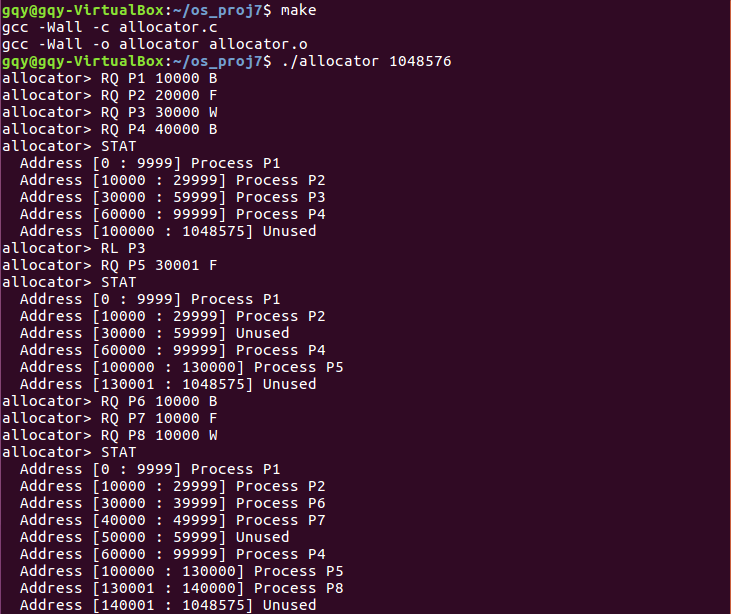
\includegraphics{a1}
		\caption{allocator测试1} \label{allocator测试1}
\end{figure}
\begin{figure}[htbp]
		\centering
		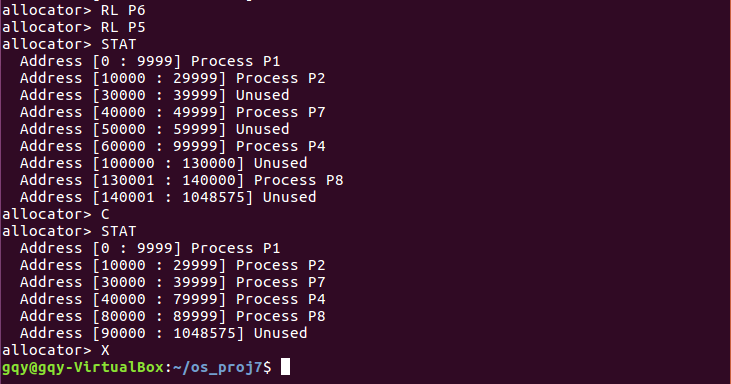
\includegraphics{a2}
		\caption{allocator测试2} \label{allocator测试2}
\end{figure}
\newpage
首先用Makefile文件编译,生成可执行文件allocator,指定内存大小1048576.然后分别分配给进程P1,P2,P3,P4内存并打印状态;释放P3,分配进程P5后打印状态;以三种分配方式分配P6,P7,P8后打印状态;释放P6,P5后打印状态;compact指令整理后再次打印状态;最后退出。测试结果如图 \ref{allocator测试1}和图 \ref{allocator测试2}。
\end{itemize}
\section{Conclusion}

\subsection{问题与解决方案}
本次project7主要实现了连续内存分配的管理,连续内存空间分配的三种分配策略理解上比较简单,程序的实现整体上难度也不大。实验中比较重要的地方在于内存分配链表的维护,但只要编程仔细保持清醒的头脑就可以顺利完成。

\subsection{实验心得}
本次project7顺利实现了连续内存分配管理与维护,虽然难度不大但是再设计内存分配链表以及实现各种分配算法的时候还是要考虑全面,谨慎操作,否则很容易出错。总的来说本次project让我熟悉了数据结构的使用,锻炼了程序设计能力也进一步加深了我对内存管理的理解。



%----------------------------------------------------------------------------------------


\end{document}